\documentclass{article}
\usepackage[utf8]{inputenc}
\usepackage{amsmath}
\usepackage{amsthm}
\usepackage{bm}
\usepackage{wrapfig}
\usepackage{graphicx}
\usepackage[a4paper, total={6in, 8in}]{geometry}

\graphicspath{ {extras/} }

% per usare la r corsiva di griffiths
% punti esclamativi per togliere lo spazio extra strano
\def\rcurs{{\mbox{$\resizebox{.16in}{.08in}{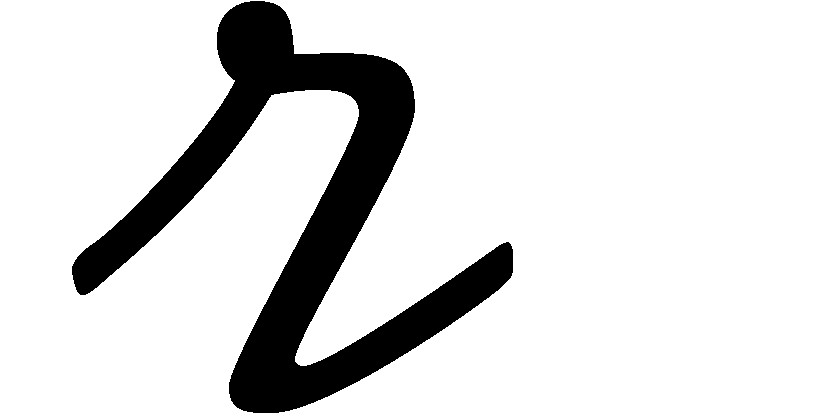
\includegraphics{ScriptR}}$}} \!\!}
\def\brcurs{{\mbox{$\resizebox{.16in}{.08in}{
\includegraphics{BoldR}}$}}}
\def\hrcurs{{\mbox{$\hat \brcurs$}} } 

\renewcommand{\epsilon}{\varepsilon}
\newcommand{\mbf}{\mathbf}
\newcommand{\vers}[1]{\mbf{\hat #1 }}
\newcommand{\qpe}[1][1]{ \frac{ #1 }{ 4\pi\epsilon_0 } }

\numberwithin{equation}{section}

\title{ Electromagnetism }
\author{William Luciani}
\date{July 2021}

\begin{document}

\maketitle

\tableofcontents

\pagebreak


\section{Costanti} % (fold)
\label{sec:costanti}

\begin{align}
    \epsilon_0  &= 8.85     \cdot 10^{-12}  \; \mathrm{ C^2 / N m^2 }\\
    e           &= 1.6      \cdot 10^{-19}  \; \mathrm{ C }\\
\end{align}

% section costanti (end)

\section{Strumenti matematici} % (fold)
\label{sec:strumenti_matematici}

\subsection{Vettori} % (fold)
\label{sub:vettori}

Prodotto misto: 

\begin{equation}
    \mbf{ A \cdot ( B \times C ) }
\end{equation}
è possibile ciclare i tre vettori
\begin{equation}
    \mbf{ A \cdot ( B \times C ) } =
    \mbf{ B \cdot ( C \times A ) } =
    \mbf{ C \cdot ( A \times B ) }
\end{equation}
e anche scambiare prodotto scalare e vettoriale
\begin{equation}
    \mbf{ A \cdot ( B \times C ) } = \mbf{ ( A \times B ) \cdot C }
\end{equation}

Doppio prodotto vettore. Vale la regola del BAC-CAB:

\begin{equation}
    \mbf{ A \times ( B \times C ) } = \mbf{ B ( A \cdot C) - C ( A \cdot B) }
\end{equation}
Non è associativo ma vale l'identità di Jacobi:
\begin{equation}
    \mbf{ A \times ( B \times C ) } +
    \mbf{ B \times ( C \times A ) } +
    \mbf{ C \times ( A \times B ) } = 0
\end{equation}

% subsection vettori (end)

\subsection{Analisi Vettoriale} % (fold)
\label{sub:analisi_vettoriale}



Derivazione in coordinate cartesiane. Operatore nabla:
\begin{equation}
    \nabla = \partial_x \vers x + \partial_y \vers y + \partial_z \vers z
\end{equation}

Gradiente: 
\begin{equation}
    \nabla f = \partial_x f \vers x + \partial_y f \vers y + \partial_z f \vers z
\end{equation}

Rotore: 
\begin{equation}
    \nabla \times \mbf A = 
    \begin{vmatrix}
        \vers i     & \vers j       & \vers k       \\
        \partial_x  & \partial_y    & \partial_z    \\
        A_x         & A_y           & A_z
    \end{vmatrix}
\end{equation}

Divergenza: 
\begin{equation}
    \nabla \cdot \mbf A = \partial_x A_x + \partial_y A_y + \partial_z A_z
\end{equation}


\subsubsection{Gradiente} % (fold)
\label{ssub:gradiente}


Il gradiente può anche essere definito nel seguente modo, indipendente dalle coordinate usate.
\begin{equation} \label{eq:grad_def}
    ( \nabla f ) \cdot \vers t = \lim_{ dl \to 0 }  \frac{ df }{ dl } 
\end{equation}
Dove la variazione di f è presa lungo un tratto infinitesimo di lunghezza $dl$ e direzione $\vers t$.

Passando ad un percorso finito $\gamma$ si ha 
\begin{equation*}
    \int_\gamma ( \nabla f ) \cdot \vers t dl = \Delta f
\end{equation*}

Questo è il teorema del gradiente (o teorema fondamentale del calcolo), che può esser scritto anche nel seguente modo.
\begin{equation}
    \int_A^B \nabla f \cdot d \mbf l = f(B) - f(A)
\end{equation}

Per il gradiente c'è un modo più immediato di trovare la relazione sopra, ma il modo sopra è utile poichè è del tutto analogo al procedimento per il rotore e la divergenza.

Il modo più diretto è il seguente. Il differenziale di un campo vettoriale scalare può esser scritto nel seguente modo:
\begin{equation}
    df = \nabla f \cdot d \mbf l
\end{equation}
Integrando segue direttamente il teorema del gradiente.

% subsubsection gradiente (end)

\subsubsection{Rotore} % (fold)
\label{ssub:rotore}

Per il rotore vale la seguente definizione:
\begin{equation} \label{eq:rot_def}
    ( \nabla \times \mbf A ) \cdot \vers n 
        = \lim_{ dS \to 0 } \frac{ 1 }{ dS }  \int_\gamma \mbf A \cdot d \mbf l 
        = \lim_{ dS \to 0 } \frac{ dC }{ dS }
\end{equation}
Dove $dS$ è un'area infinitesima e $\vers n$ è la sua normale. $\gamma$ è il bordo di S, ovvero un circuito infinitesimo. $dC$ è la circuitazione attraverso questo circuito infinitesimo.

Passando ad una superficie $S$ finita si ha quindi:
\begin{equation*}
    \int_S ( \nabla \times \mbf A ) \cdot \vers n dS = C
\end{equation*}
Questo è il teorema di Stokes (o del rotore), che può esser scritto anche nel seguente modo. ($\partial S$ è il bordo di $S$)
\begin{equation}
    \int_S ( \nabla \times \mbf A ) \cdot d \mbf S = \int_{\partial S} \mbf A \cdot d \mbf l
\end{equation}


% subsubsection rotore (end)

\subsubsection{Divergenza} % (fold)
\label{ssub:divergenza}


Per la divergenza vale la seguente definizione:
\begin{equation}    \label{eq:div_def} 
    \nabla \cdot \mbf A 
        = \lim_{ dV \to 0 } \frac{ 1 }{ dV } \int_S \mbf A \cdot d \mbf S 
        = \lim_{ dV \to 0 } \frac{ d\Phi }{ dV }
\end{equation}
Dove $dV$ è un volume infinitesimo, $S$ è la sua superficie. $d\Phi$ è il flusso attraverso $S$.

Passando ad un volume finito si ha:
\begin{equation*}
    \int_V \nabla \cdot \mbf A dV = \Phi
\end{equation*}
Questo è il teorema della divergenza (o di Gauss), che può esser scritto anche nel seguente modo. ($\partial V$ è il bordo di $V$)
\begin{equation}
    \int_V \nabla \cdot \mbf A dV = \int_{\partial V} \mbf A \cdot d \mbf S
\end{equation}


% subsubsection divergenza (end)

\subsection{Derivate seconde} % (fold)
\label{sub:derivate_seconde}

Si possono fare le seguenti derivate seconde con l'operatore nabla:
\begin{enumerate}
    \item $\nabla \times \nabla f = 0 $ 
    \item $\nabla \cdot \nabla f =: \nabla^2 f = \Delta f$ Definizione del Laplaciano
    \item $\nabla \times \nabla \times A$ 
    \item $\nabla \cdot \nabla \times A = 0$ 
    \item $\nabla (\nabla \cdot A)$ 
\end{enumerate}
La 5. non è di particolare interesse e per la 3 vale la seguente uguaglianza:
\begin{equation}
    \nabla \times \nabla \times A = \nabla (\nabla \cdot A) - \nabla^2 A
\end{equation}
Per chiarezza esplicitiamo il laplaciano di un campo scalare e di un campo vettoriale:
\begin{align}
    \nabla^2 f &= \partial_x^2 f + \partial_y^2 f + \partial_z^2 f \\
    \nabla^2 A &= \nabla^2 A_x \vers x + \nabla^2 A_y \vers y + \nabla^2 A_z \vers z
\end{align}

% subsection derivate_seconde (end)

\subsection{Derivate utili} % (fold)
\label{sub:derivate_utili}

\begin{align}
    \nabla \cdot \frac{ \vers r }{ r^2 } &= 4 \pi \delta(\mbf r) \\
    \nabla \cdot (r^n \vers r)  &= (n+2)r^{n-1}, \qquad n \neq -2\\
    \nabla r^n &= n r^{n-1} \vers r \\
    \nabla \times (r^n \vers r) &= 0
\end{align}

% subsection derivate_utili (end)

% subsection analisi_vettoriale (end)

% section strumenti_matematici (end)



\section{Elettrostatica nel vuoto} % (fold)
\label{sec:elettrostatica_nel_vuoto}

\subsection{Formule Sperimentali} % (fold)
\label{sub:formule_sperimentali}

\begin{equation}
    \brcurs = \mbf r - \mbf r'
\end{equation}
Dove r è il punto in cui vogliamo calcolare il campo e r' è la posizione della carica. (Se pensiamo alla forza, r è la posizione della carica su cui calcoliamo la forza, r' è l'altra).

\begin{equation}
    \mbf{F} = \frac{1}{4 \pi \epsilon_0 } \frac{q_1 q_2}{\rcurs^2} \hrcurs
\end{equation}

\begin{equation}
    \mbf{E} = \lim_{q \to 0} \frac{\mbf F}{q}
\end{equation}
Limite non matematico ma fisico, pensiamo di avere una carica di prova molto piccola in modo che non alteri le cariche che generano il campo.

\begin{equation}
    \mbf{E} = \frac{1}{4 \pi \epsilon_0 } \frac{q}{\rcurs^2} \hrcurs
\end{equation}

Principio di sovrapposizione:
\begin{equation}
    \mbf E_{tot} = \mbf E_1 + \mbf E_2 + \dots
\end{equation}

Distribuzioni di carica:

\begin{equation}
    dq = \lambda dl = \sigma dS = \rho d\tau
\end{equation}

Dal principio di sovrapposizione:
\begin{equation}
    \mbf{E} = \frac{1}{4 \pi \epsilon_0 } \int          \frac{dq}           {\rcurs^2} \hrcurs
            = \frac{1}{4 \pi \epsilon_0 } \int_\gamma   \frac{\lambda dl}   {\rcurs^2} \hrcurs
            = \frac{1}{4 \pi \epsilon_0 } \int_S        \frac{\sigma dS}    {\rcurs^2} \hrcurs
            = \frac{1}{4 \pi \epsilon_0 } \int_V        \frac{\rho d\tau}   {\rcurs^2} \hrcurs
\end{equation}

% subsection formule_sperimentali (end)

\subsection{Teorema di Gauss e prima equazione di Maxwell nel vuoto} % (fold)
\label{sub:teorema_di_gauss_e_prima_equazione_di_maxwell}

% subsection teorema_di_gauss_e_prima_equazione_di_maxwell (end)

Teorema di Gauss:
\begin{equation} \label{eq:gauss_int} 
    \Phi ( \mbf E ) = \int_S \mbf{ E \cdot \hat n} \, dS = \frac{ Q_{int} }{ \epsilon_0 } 
\end{equation}

\begin{proof}
    Pensiamo ad una singola carica $q$ posta nell'origine. Questo non lede alla generalità poiché se non è nell'origine possiamo traslarla e se abbiamo più cariche vale il principio di sovrapposizione e quindi il flusso totale è la somma dei singoli flussi. Abbiamo quindi:

    \begin{equation*}
        \Phi ( \mbf E ) = \frac{q}{4 \pi \epsilon_0 } \int_S \frac{ \vers r  \cdot \vers n dS }{ r^2 }
                        = \frac{q}{4 \pi \epsilon_0 } \int_S \frac{ dS_r }{ r^2 } 
                        = \frac{q}{4 \pi \epsilon_0 } \int d\Omega
                        = \frac{q}{\epsilon_0 }
    \end{equation*}

\end{proof}

Per scrivere il teorema di Gauss in forma differenziale vogliamo mostrare che vale l'equazione \ref{eq:div_def}
\begin{proof}
    Pensiamo ad un cubetto infinitesimo con assi paralleli agli assi cartesiani. Esso ha un vertice in $(x, y, z)$ e il vertice opposto in $(x + dx, y + dy, z + dz)$. Pensiamo al flusso attraverso le due facce ortogonali all'asse x:
    \begin{equation*}
        d\Phi_x = E_x(x + dx, y, z) dydz - E_x(x, y, z) dydz = \partial_x E_x dxdydz = \partial_x E_x dV
    \end{equation*}
    E varranno formule analoghe per le altre facce. Il flusso totale è quindi:
    \begin{equation*}
        d\Phi = (\partial_x E_x + \partial_y E_y + \partial_z E_z) dV = (\nabla \cdot \mbf E ) dV
    \end{equation*}
    quindi si ha:
    \begin{equation*}
        \nabla \cdot \mbf E 
        = \lim_{ dV \to 0 } \frac{ d\Phi }{ dV }
    \end{equation*}
    che è la tesi.
\end{proof}

Applicando questo teorema alla \ref{eq:gauss_int} si ha:
\begin{equation}
    \int_{\partial V} \mbf E \cdot d \mbf S = \int_V \nabla \cdot \mbf E dV = \int_V \frac{ \rho }{ \epsilon_0 } 
\end{equation}
Ma il volume di integrazione è del tutto arbitrario, per cui si ha:
\begin{equation} \label{eq:gauss_diff} 
    \nabla \cdot \mbf E = \frac{ \rho }{ \epsilon_0 } 
\end{equation}
Che è il teorema di Gauss in forma differenziale ovvero la prima equazione di Maxwell nel vuoto. 

\subsection{Seconda equazione di Maxwell nel vuoto} % (fold)
\label{sub:seconda_equazione_di_maxwell_nel_vuoto}

Pensando al campo generato da una carica puntiforme si può vedere che il campo elettrico è conservativo, in quanto si trova:
\begin{equation}
    \int_A^B \mbf E \cdot d \mbf l 
        = \qpe \int_A^B \frac{ Q }{ r^2 } \vers r \cdot d \mbf l 
        = \qpe[Q] \int_A^B \frac{ 1 }{ r^2 } dr
        = \qpe[Q] \left ( \frac{ 1 }{ r_A } - \frac{ 1 }{ r_B } \right )
        = V(A) - V(B)
\end{equation}
Ovvero l'integrale di linea dipende solo dagli estremi e si può scrivere:
\begin{equation}
    \mbf E = - \nabla V
\end{equation}
Ma ricordando che il rotore del gradiente è nullo si ha:
\begin{equation} \label{eq:rot_E_stat} 
    \nabla \times \mbf E = 0
\end{equation}

Un modo per mostrare che il rotore del gradiente è nullo è di applicare il teorema di Stokes ad una superficie qualsiasi:
\begin{equation}
    \int_S ( \nabla \times \nabla f ) \cdot d \mbf S = \int_{\partial S} \nabla f \cdot d \mbf l = f(A) - f(A) = 0
\end{equation}
Per l'arbitrarietà di $S$ si ha quindi che
\begin{equation}
    \nabla \times \nabla f = 0
\end{equation}

DIM STOKES BALZATA

% subsection seconda_equazione_di_maxwell_nel_vuoto (end)

\subsection{Dipolo} % (fold)
\label{sub:dipolo}

Carica $+q$ e carica $-q$ a distanza $\delta$. Vettore $\pmb \delta$ dalla carica negativa a quella positiva. $\mbf p$ momento di dipolo.
\begin{equation}
    \mbf p = q \pmb \delta
\end{equation}

Calcoliamo il potenziale ad $r >> \delta$. $r_+$ distanza dalla carica positiva, $r_-$ distanza dalla carica negativa. 
\begin{equation}
    V(\mbf r) = \qpe[q] \left ( \frac{ 1 }{ r_+ } - \frac{ 1 }{ r_- }  \right )
\end{equation}
Usando il teorema del coseno ed espandendo in serie di Taylor: ($\alpha$ è l'angolo tra il vettore posizione $\mbf r$ e $\mbf p$, dove r è preso dal centro del dipolo)
\begin{equation}
    \frac{ 1 }{ r_\pm } 
        = \frac{ 1 }{ r \sqrt{ 1 + (\delta/2r)^2 \mp \frac{\delta}{r} \cos \alpha} } 
        \sim \frac{ 1 }{ r \sqrt{ 1 \mp \frac{\delta}{r} \cos \alpha} } 
        \sim \frac{ 1 \pm \frac{\delta}{2r} \cos \alpha }{ r } 
\end{equation}
Quindi si ha:
\begin{equation}
    V(\mbf r) 
        = \qpe[q] \frac{ \delta \cos \alpha }{ r^2 } 
        = \qpe[q \delta \cos \alpha] \frac{ 1 }{ r^2 } 
        = \qpe[\mbf p \cdot \vers r] \frac{ 1 }{ r^2 } 
\end{equation}

Applicando il gradiente a questa espressione si può poi trovare il campo elettrico. Si ha 
\begin{align*}
    \nabla \left ( \frac{ \mbf p \cdot \mbf r }{ r^3 } \right ) 
    &= \frac{ \nabla(\mbf p \cdot \mbf r) }{ r^3 } + \mbf p \cdot \mbf r \nabla \left ( \frac{ 1 }{ r^3 } \right ) \\
    \nabla (\mbf p \cdot \mbf r) &= \mbf p \\
    \nabla \left ( \frac{ 1 }{ r^3 } \right ) &= -3 \frac{ \vers r }{ r^4 } \\
    \nabla \left ( \frac{ \mbf p \cdot \mbf r }{ r^3 } \right )  &= \frac{ \mbf p }{ r^3 } - \frac{ 3 ( \mbf p \cdot \vers r) \vers r}{ r^3 }
\end{align*}
Da cui si ha 
\begin{equation}
    E(\mbf r) = -\nabla V = \qpe \frac{ 1 }{ r^3 } ( 3 ( \mbf p \cdot \vers r) \vers r  -  \mbf p )
\end{equation}

Si può poi mostrare che un dipolo in un campo elettrico $\mbf E$ è sottoposto alla seguente forza:
\begin{equation}
    \mbf F = (\mbf p \cdot \nabla ) \mbf E = \nabla ( \mbf{ p \cdot E })
\end{equation}
Ha la seguente energia potenziale:
\begin{equation}
    U = - \mbf{p \cdot E}
\end{equation}
Subisce il seguente momento torcente:
\begin{equation}
    \mbf{ M = p \times E}
\end{equation}

DIM BALZATE

% subsection dipolo (end)

\subsection{Espansione multipoli} % (fold)
\label{sub:espansione_multipoli}

% subsection espansione_multipoli (end)

\subsection{Conduttori} % (fold)
\label{sub:conduttori}

% subsection conduttori (end)

\subsection{condensatori(?)} % (fold)
\label{sub:condensatori}

% subsection condensatori (end)

\subsection{Energia e pressione} % (fold)
\label{sub:energia_e_pressione}

% subsection energia_e_pressione (end)

\subsection{Equazione di Poisson} % (fold)
\label{sub:equazione_di_poisson}

% subsection equazione_di_poisson (end)

% section elettrostatica_nel_vuoto (end)

\section{Elettrostatica nei materiali} % (fold)
\label{sec:elettrostatica_nei_materiali}

% section elettrostatica_nei_materiali (end)

\section{Correnti} % (fold)
\label{sec:correnti}

% section correnti (end)

\end{document}
